\documentclass[12pt,letter]{article}


\usepackage{nicefrac,amsmath}
\usepackage[english]{babel}
\usepackage{helvet}
\usepackage{enumerate}
\usepackage{parskip}
%\usepackage{apacite}
\usepackage[english]{babel}
\usepackage{booktabs}
\usepackage[top=1in, bottom=1in, left=1in, right=1in]{geometry}
\usepackage{graphicx}
\usepackage{subfigure}
\usepackage{url}
\usepackage{hyperref}
\usepackage{physics}
\usepackage{cancel}
\usepackage{gensymb}
\usepackage{bbm}
\usepackage{dsfont}
\usepackage{mathtools}
\usepackage{appendix}
\usepackage{etoolbox}

\usepackage{amsfonts}

% Inserts \clearpage before \begin{appendices}
\BeforeBeginEnvironment{appendices}{\clearpage}

\usepackage{algpseudocode}
\usepackage{algorithm}


\usepackage[usenames,dvipsnames]{color}
 \usepackage{listings}
 \definecolor{Brown}{cmyk}{0,0.81,1,0.60}
 \definecolor{OliveGreen}{cmyk}{0.64,0,0.95,0.40}
 \definecolor{CadetBlue}{cmyk}{0.62,0.57,0.23,0}



 \lstset{language=python,
 basicstyle=\small,
 frame=single,
 keywordstyle=\ttfamily\color{OliveGreen}\bfseries,
 identifierstyle=\ttfamily\color{CadetBlue}\bfseries, 
 commentstyle=\color{Brown}\ttfamily,
 stringstyle=\ttfamily\color{red},
 showstringspaces=false}


\newcommand{\argmax}[1]{\underset{#1}{\operatorname{arg}\,\operatorname{max}}\;}
\newcommand{\argmin}[1]{\underset{#1}{\operatorname{arg}\,\operatorname{min}}\;}



%\usepackage{cmbright}
\usepackage[T1]{fontenc}

\usepackage{xcolor}
\usepackage{mdframed}



\setlength{\parskip}{12pt} % 1ex plus 0.5ex minus 0.2ex}

%\renewcommand{\familydefault}{\sfdefault}

\setlength{\parindent}{0cm}
\renewcommand{\baselinestretch}{1.2}

\title{{\bf Numerical Approximations of Derivatives} }


\date{}
\begin{document}
\maketitle
\vspace{-1.0in}

%{\small 
%\tableofcontents
%\listoffigures
%\listofalgorithms
%}

%\newpage



\section{Overview}
\vspace{12pt}
    \begin{mdframed}[backgroundcolor=blue!20] 
        {\bf Question}: How do we calculate derivatives numerically?
    \end{mdframed}
    
Often, finding the derivatives of functions analytically can be hard. Instead, we can  approximate derivatives numerically by using discrete differences or finite differences. In fact, as long as we can evaluate the function, we can always approximate the derivative. 

\section{Derivative (numerical) approximation}


In general, there are two types of approximations for derivatives: forward (backward) differences and central differences. Both types of approximation are derived from the limit definition of derivatives.

\subsection{The forward/backward difference approximation} 
Here, we drop the limit operation to approximate the analytical derivative as:
\begin{align}
        \dv{f}{x} &= \lim_{\Delta x \rightarrow 0}\frac{\Delta f}{\Delta x} 
                      = \lim_{\Delta x \rightarrow 0}\frac{f\left(x+\Delta x\right) - f\left(x\right)}{\Delta x} \notag \\ \notag\\
                      &\approx \frac{\Delta f}{\Delta x} = \frac{f\left(x+\Delta x\right) - f\left(x\right)}{\Delta x}, 
	\label{approx1}
\end{align}		
for a small $\Delta x$. This approximation is called {\em the forward difference approximation} of the first derivative. Its analogous counterpart, the {\em backward difference}, is given by: 
\begin{align}
        \dv{f}{x} \approx \frac{\Delta f}{\Delta x} = \frac{f\left(x\right)- f\left(x-\Delta x\right)}{\Delta x}.
	\label{approx2}
\end{align}
\newpage
\subsection{The central difference approximation} 
We can also use a slightly modified definition of the analytical derivative of a scalar function of a single scalar variable, which is given by: 
\begin{align}
        \dv{f}{x} = \lim_{\Delta x \rightarrow 0}\frac{\Delta f}{\Delta x} = \lim_{\Delta x \rightarrow 0}\frac{f\left(x+\Delta x\right) - f\left(x-\Delta x\right)}{2\Delta x}.
	\label{dfx2Central}
\end{align}
We can drop the limit in the calculation of Equation \ref{dfx2Central} to obtain the {\em central approximation} of the derivative which is given by:    
\begin{align}
        \dv{f}{x} \approx \frac{\Delta f}{\Delta x} \approx \frac{f\left(x+\Delta x\right) - f\left(x-\Delta x\right)}{2\Delta x}. 
	\label{dfx2CentralApprox}
\end{align}

\section{Representing function values on grids}

Numerically, the value of functions are represented as a discrete grid of values, which can be  stored in multi-dimensional arrays. The array's dimensionality depends on the type of function and on implementation decisions. For example, a scalar function of a scalar variable can be stored in a 1-D array while a scalar function of two variables can be stored in a $M\times N$ matrix (i.e., a multidimensional array). Here, $M$ is the number of rows in the matrix and $N$ is the number of columns. Similarly, a scalar function of three variables can be stored in a $M\times N \times K$ array. Figure \ref{fig_matrixFunction} illustrates the values of the Rosenbrock function stored in a $18\times 18$ matrix. 
\begin{figure}[H]
	\begin{center}
		{\includegraphics[width=.99\textwidth]{figs/matrixFunction}}
	\end{center}
	\caption{The Rosenbrock function stored in a $18 \times 18 $ matrix C.}
	\label{fig_matrixFunction}
\end{figure}

\section{Discrete derivatives on grids}

Given the matrix representation of the function, we can approximate the function's derivatives (gradient, Jacobian) by means of discrete differences.
The derivative approximation can be calculated at all points of the function's domain (if the derivative exists, of course). Figure \ref{fig_matrixFunctionSample} shows a sample region of the matrix and the function values. 
\begin{figure}[H]
	\begin{center}
		{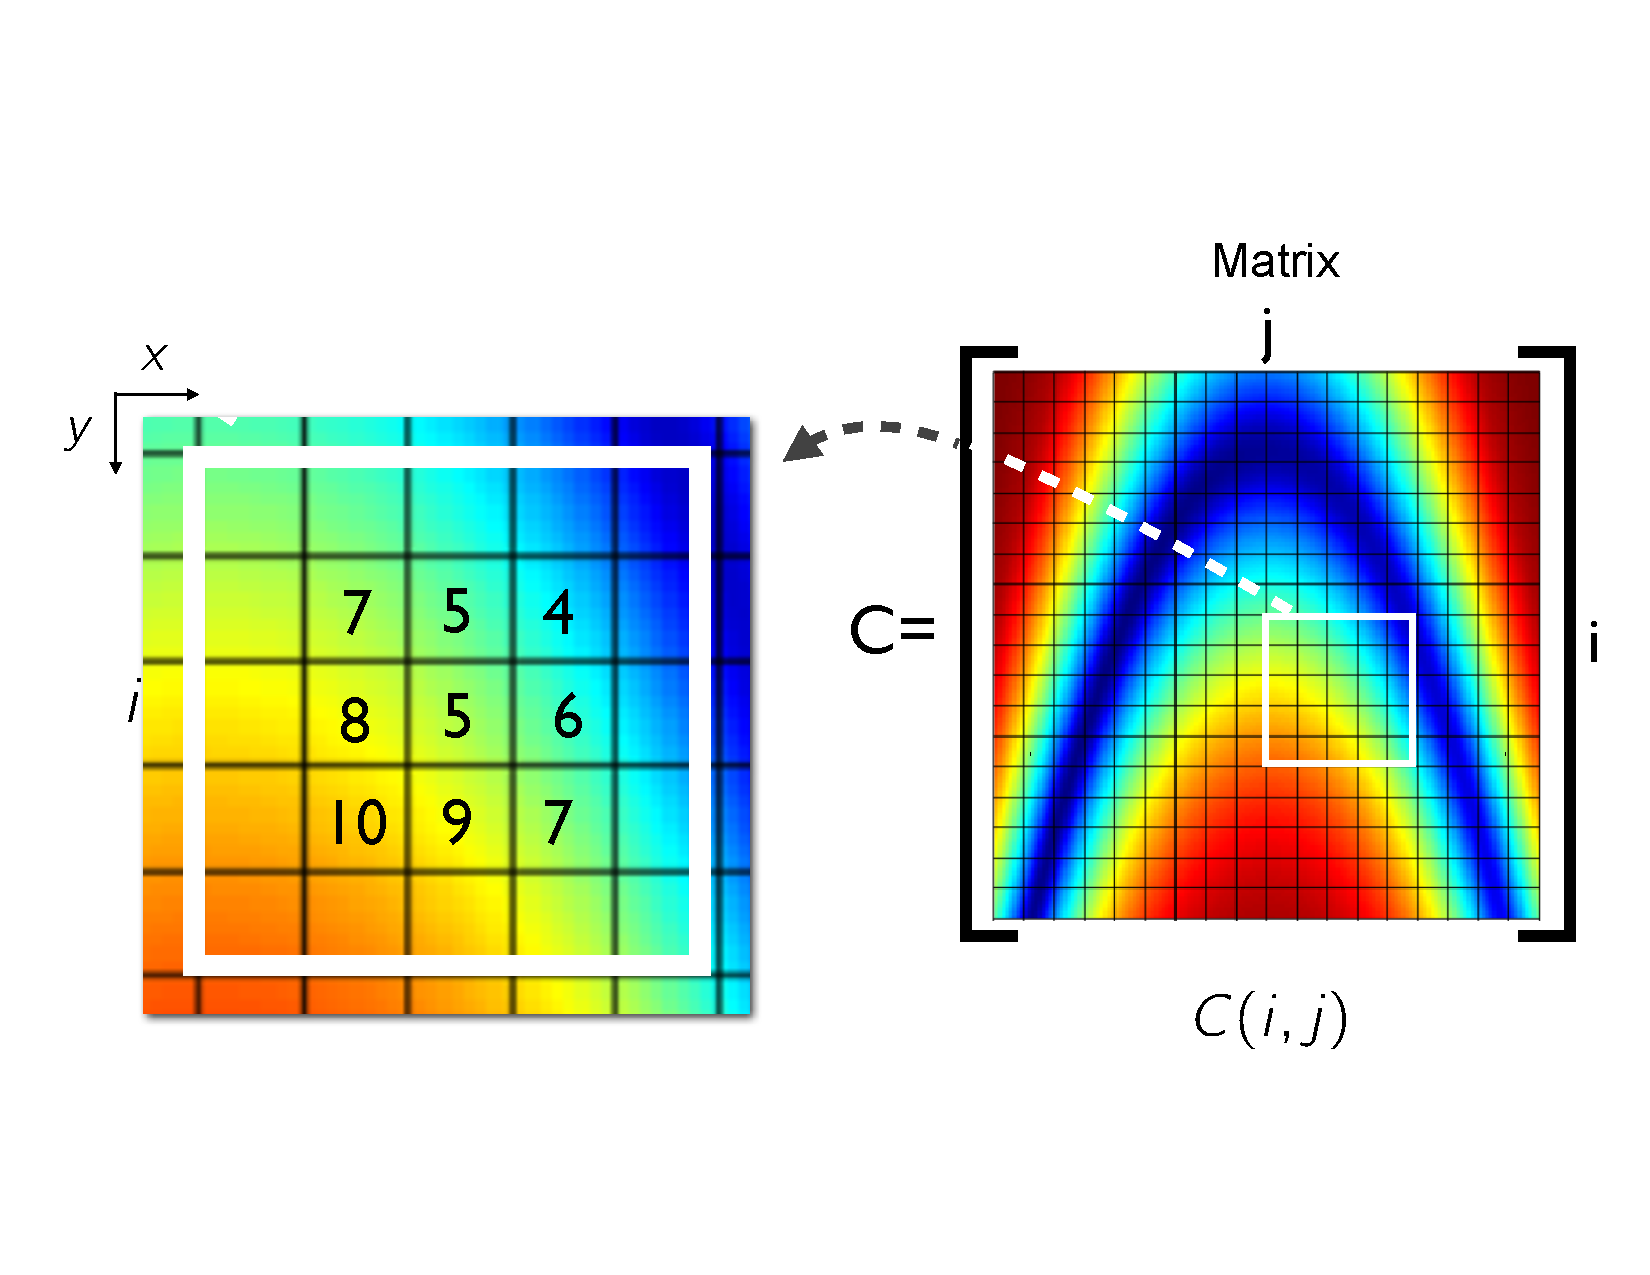
\includegraphics[width=.99\textwidth]{figs/gridSample}}
	\end{center}
	\caption{A sample region of function values from the matrix.}
	\label{fig_matrixFunctionSample}
\end{figure}

To calculate the gradient at a given position $(x,y)$, we treat the matrix as a grid of values and calculate the required derivatives using finite differences. \\\\
    \begin{mdframed}[backgroundcolor=yellow!20] 
        {\bf Important}: When working with Cartesian coordinate systems and multi-dimensional arrays, be aware of the relationship between array indices $(i,j)$ and Cartesian coordinates $(x,y)$ as they are not the same!
    \end{mdframed}


\newpage
When calculating the derivative's discrete approximations, we need to convert between the Cartesian coordinates and their corresponding locations in the matrix indexing system, which uses $(i,j)$ for (row,column) indexing. We also need to be aware of the location of the origin of the Cartesian coordinate that we are using, e.g., the $(x,y)=(0,0)$ is at the top-left corner of the coordinate system with the y-axis pointing downwards,  the $(x,y)=(0,0)$ is at the bottom-left corner of the coordinate system and the y-axis points upwards. Two examples of these grid representations are shown in Figure \ref{fig_grid}.
\begin{figure}[H]
	\begin{center}
		{\includegraphics[width=.99\textwidth]{figs/gridFinite}}
	\end{center}
	\caption{Matrix indexing vs. Cartesian coordinates.}
	\label{fig_grid}
\end{figure}

Figure \ref{fig_whole} shows a graphical overview of the gradient calculation using central derivatives.
\begin{figure}[H]
	\begin{center}
		{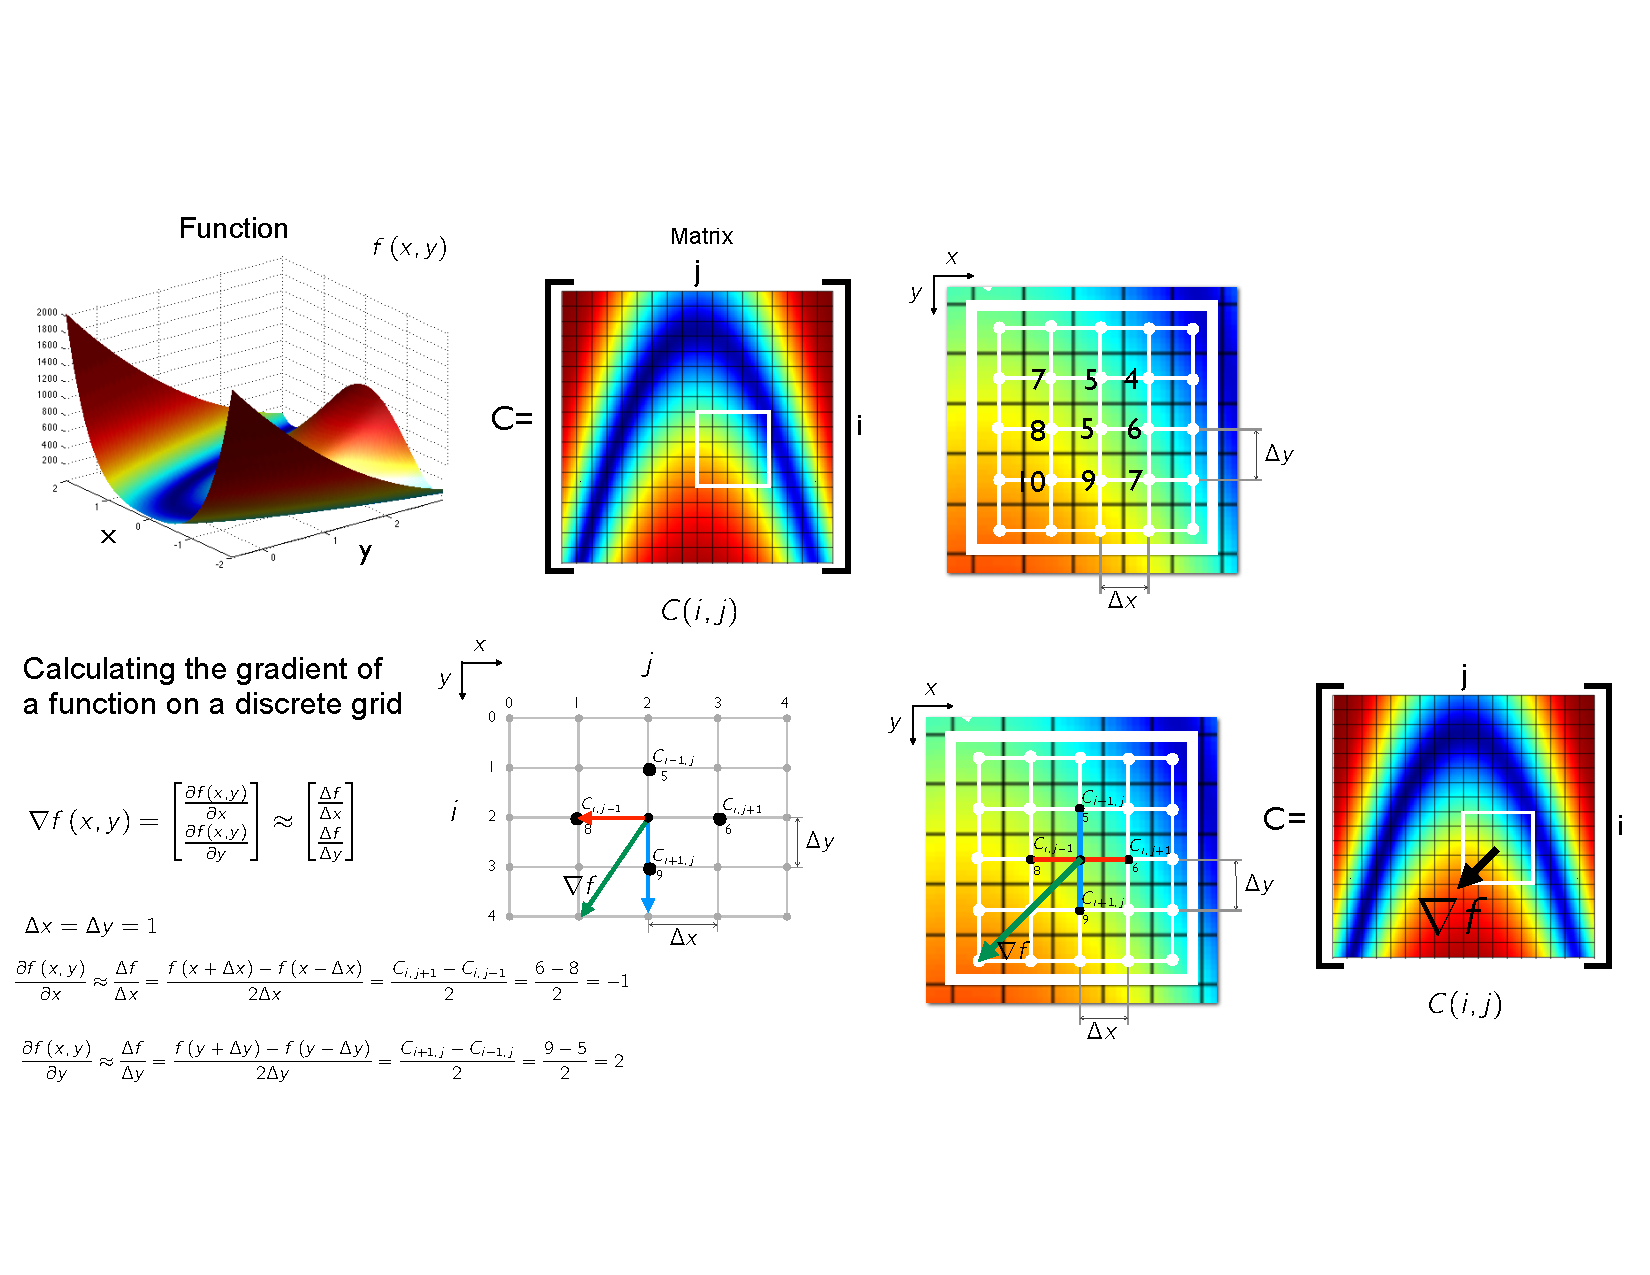
\includegraphics[angle=90, width=.78\textwidth]{figs/discreteCalculationWhole}}
	\end{center}
	\caption{Gradient approximation using central differences.}
	\label{fig_whole}
\end{figure}

%% References 
\bibliographystyle{unsrt} 
\bibliography{refs}

\end{document}
% end of file template.tex

\newpage


%$(i,j) \leftrightarrow (y,x)$
%
%$(i,j) \leftrightarrow (M-y,x)$
%
%$0\,\,\,1\,\,\,2$
%
%$(M,N)$
%


%\begin{align}
%        \dv{f}{x} \approx \frac{\Delta f}{\Delta x} \approx \frac{f\left(x+\Delta x\right) - f\left(x-\Delta x\right)}{2\Delta x}. \\\\
%                \dv{f}{y} \approx \frac{\Delta f}{\Delta y} \approx \frac{f\left(y+\Delta y\right) - f\left(y-\Delta y\right)}{2\Delta y}. 
%%	\label{dfx}
%\end{align}
%
%\begin{align}
%        %\dv{f}{\bf x} = \pdv{f}{\left(x_1, x_2, \dots, x_N\right)}  
%        \grad f \left(x,y\right) = 
%        \begin{bmatrix}
%        \pdv{f\left(x,y\right)}{x}\\
%        \pdv{f\left(x,y\right)}{y}
%        	\end{bmatrix}
%	\approx
%        \begin{bmatrix}
%        	 \frac{\Delta f}{\Delta x}\\
%         \frac{\Delta f}{\Delta y}
%        	\end{bmatrix}	
%\end{align}	
%
\begin{align}
        \Delta x = \Delta y = 1\\\\
        %\dv{f}{\bf x} = \pdv{f}{\left(x_1, x_2, \dots, x_N\right)}  
        \pdv{f\left(x,y\right)}{x} \approx  \frac{\Delta f}{\Delta x} = \frac{f\left(x+\Delta x\right) - f\left(x-\Delta x\right)}{2\Delta x} = \frac{C_{i,\,j+1} - C_{i,\,j-1}}{2} = \frac{6-8}{2} =  -1
\end{align}	
\begin{align}
        %\dv{f}{\bf x} = \pdv{f}{\left(x_1, x_2, \dots, x_N\right)}  
       \pdv{f\left(x,y\right)}{y} \approx  \frac{\Delta f}{\Delta y} = \frac{f\left(y+\Delta y\right) - f\left(y-\Delta y\right)}{2\Delta y} = \frac{C_{i+1,\,j} - C_{i-1,\,j}}{2} = \frac{9-5}{2} = 2
\end{align}	
%
%
%\begin{align}
%        %\dv{f}{\bf x} = \pdv{f}{\left(x_1, x_2, \dots, x_N\right)}  
%        \grad C \left(x,y\right) \approx  \grad C_{j,i} = 
%        \begin{bmatrix}
%        -1\\
%        2
%        	\end{bmatrix}
%\end{align}
%
%
%$C(i,j)$





